\chapter{Calculation of Condensed Field}

\section{Finding the Condensate of the Freeze-Out Surface}

The freeze-out surface is invariant under rotations (= independent of polar angle $\varphi$) around the collision axis and longitudinal boosts (= independent of rapidity $\eta_s$) and hence parametrized by a one-dimensional curve in the $r\text{-}\tau$-plane. The curve itself may be parametrized by some real parameter $\alpha$, following some mapping $s\mapsto (r(\alpha),\tau(\alpha))$. From the hydro simulation we wish to identify the gradient $\partial_\mu\vartheta\sim u_\mu$ of the complex phase of the condensate field with the fluid $4$-velocity $u_\mu$, hence in order to find the phase of the field, an integration of $\partial_\mu\vartheta$ over the hypersurface is needed and an integration constant $\vartheta_0$ can be chosen freely. Choose $\alpha=\arctan(y/x)$ to be the polar angle of the point $(r(\alpha),\tau(\alpha))$ in the $r\text{-}\tau$-plane. Since $r,\tau>0$ $\alpha$ is restricted to the range $[0,\pi]$ and $\vartheta(\alpha)$ on the hypersurface can be calculated via
\begin{equation}
    \vartheta(\alpha)=\vartheta_0+\int_0^\alpha\dt s\frac{\dt\vartheta}{\dt s}=\vartheta_0+\int_0^\alpha\dt s\frac{\partial x^\mu(s)}{\partial s}\partial_\mu\vartheta
\end{equation}
$\partial x^\mu(s)/\partial s$ represents the tangent vector of the freeze-out surface.

The energy density $\epsilon$ and $4$-velocity $u^\mu$ of the fluid is related to the condensate phase and density via
\begin{subequations}
    \begin{gather}
        -(\partial_\mu\vartheta)(\partial^\mu\vartheta)=\chi^2=\frac{-\mu^2+\sqrt{6\epsilon\lambda+2\mu^4}}{3}\\
        \partial^\mu\vartheta=\chi u^\mu\,,\qquad\rho^2=\sqrt{\frac{\chi^2+\mu^2}{\lambda}}
    \end{gather}
\end{subequations}
One may use the relations \eqref{eq:LinearSigmaModel_CouplingsMassesRelation} to rewrite the above equation in terms of the particle masses and the pion decay constant $f_\pi\equiv v$.
\begin{equation}
    \chi^2=\frac{-m_\sigma^2/2+\sqrt{3\epsilon m_\sigma^2/f_\pi+m_\sigma^4/2}}{3}=\frac{-m_\sigma^2+m_\sigma\sqrt{12\epsilon/f_\pi+2m_\sigma^2}}{6}\,,\qquad\rho=\sqrt{f_\pi\frac{2\chi^2+m_\sigma^2}{m_\sigma^2}}
\end{equation}

In Milne coordinates $(x^\mu)=(\tau,r,\varphi,\eta_s)$ the $4$-velocity has components $(u^\mu)=(\gamma,\gamma v,0,0)$, where $v=v(\alpha)$ is a function on the freeze-out surface.

Questions to Andreas regarding numerics:
\begin{itemize}
    \item Why is $\dt\alpha=\alpha_{j+1}-\alpha_{j}\neq\const$?
\end{itemize}

\section{Finding the Spectrum at the Detector Surface}

In general the particle number $N$ and particle number density $n(\mathbf{x})$ in position space and $n(\mathbf{p})$ in momentum space associated to the condensate $\phi(\mathbf{x})$ of a complex scalar field are given by the relations
\begin{subequations}
    \begin{gather}
        n(\mathbf{x})=\phi(\mathbf{x})\phi^*(\mathbf{x})\,,\qquad n(\mathbf{p})=\phi(\mathbf{p})\phi^*(\mathbf{p})\\
        N=\int\dt^3xn(\mathbf{x})=\int\frac{\dt^3p}{(2\pi)^3}n(\mathbf{p})
    \end{gather}
\end{subequations}
with the convention $\phi(\mathbf{x})=\int\dt^3p/(2\pi)^3\phi(\mathbf{p})e^{-\imagu\mathbf{p}\mathbf{x}}$ for the Fourier transform.



% The field configuration found by this translation prescription is then propagated forwards in time by means of the retarded Greens function
% \begin{equation}
%     \overline{\phi}(x)=\langle\phi_a(x)\rangle=\int\dt^dyG_{\text{ret}}(x,y)j(y)
% \end{equation}
% $j(y)$ is defined to be the field configruation on the freezout surface. The retarded Greens function is given by $G_{\text{ret}}(x,y)=\Theta(x^0-y^0)\big(D(x-y)-D(y-x)\big)$ where
% \begin{equation}
%     D(\Delta x)=\int\frac{\dt^3p}{(2\pi)^3}\frac{1}{2\omega_\mathbf{p}}e^{-\imagu(\omega_\mathbf{p}\Delta t-\mathbf{p}\Delta\mathbf{x})}
% \end{equation}
% and $\omega_\mathbf{p}=\sqrt{m^2+\mathbf{p}^2}$.

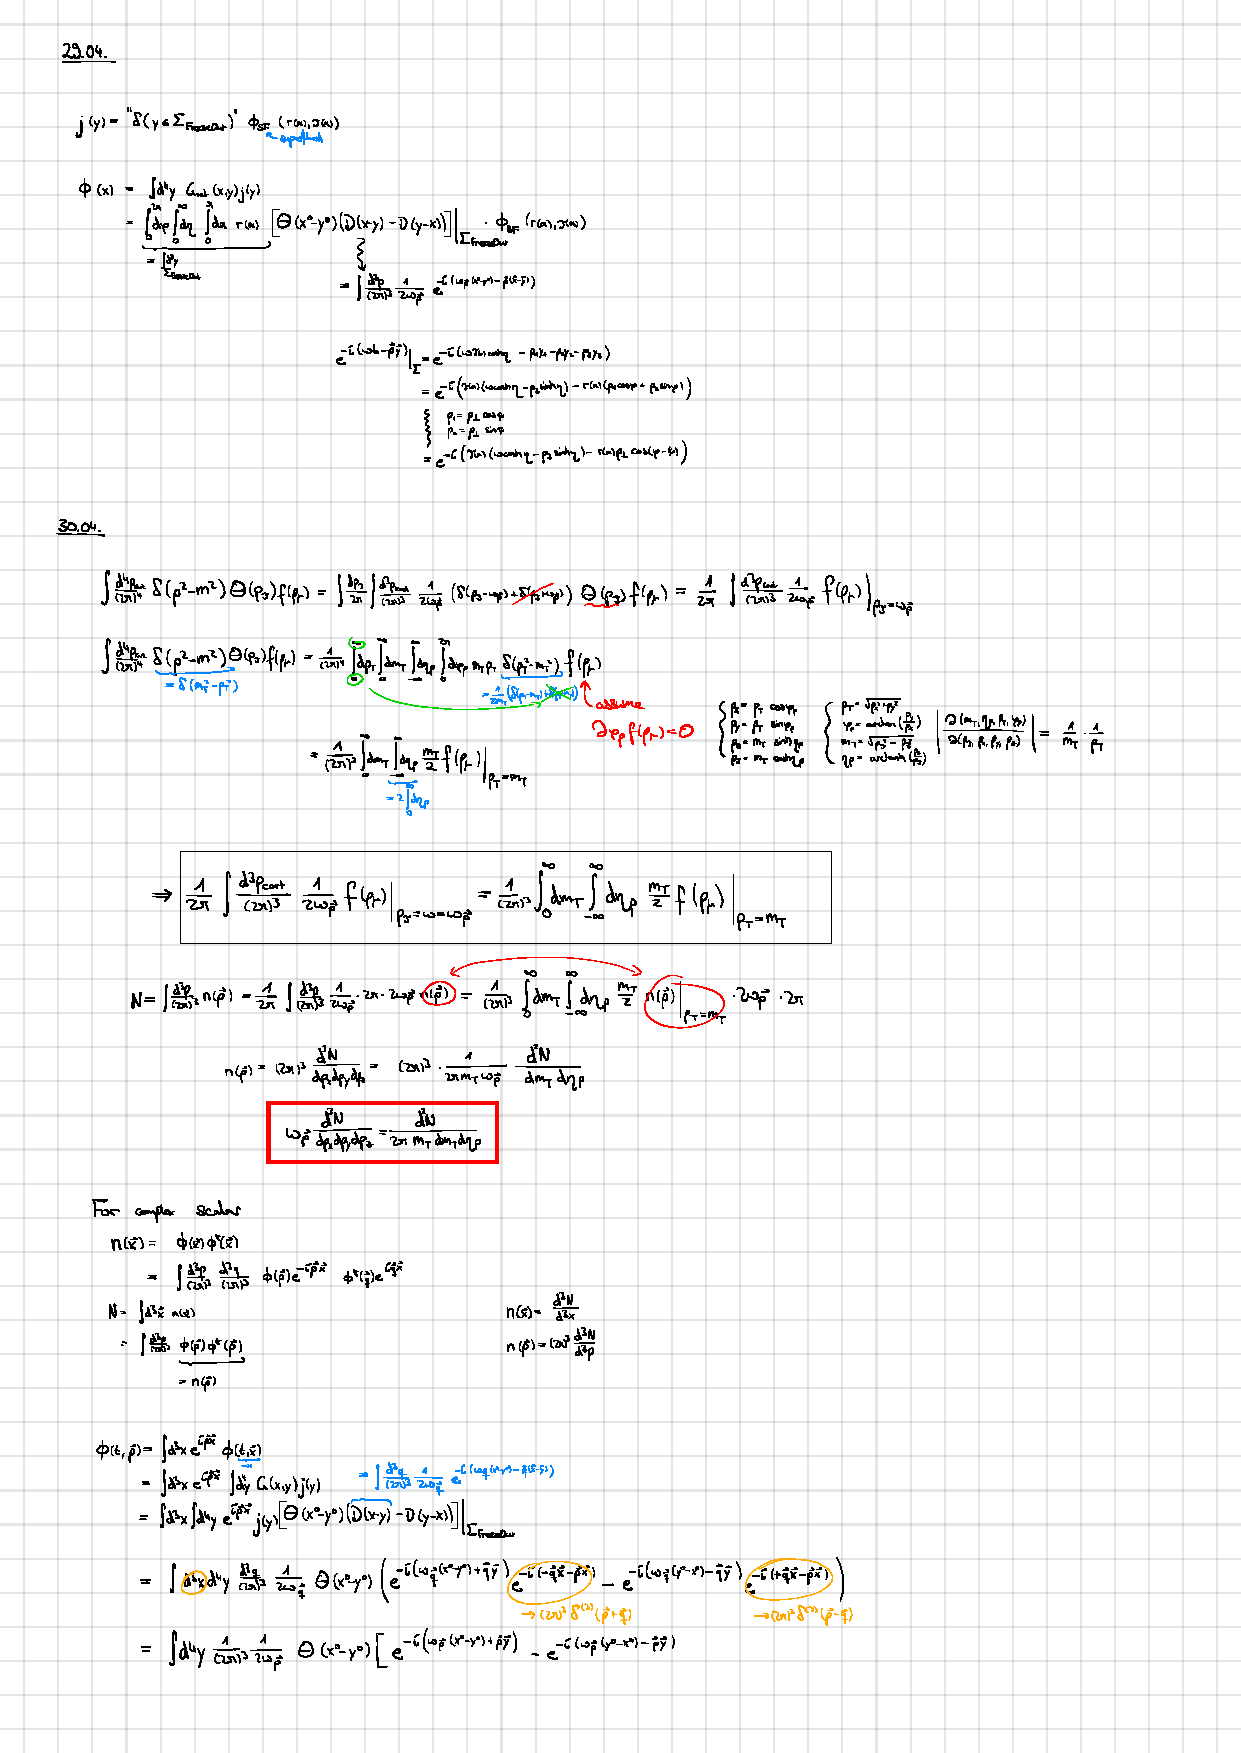
\includepdf{resources/notes_0430.pdf}

Let's evaluate the Fourier transform of the condensate field. The calculation uses the result from linear response theory
\begin{subequations}
    \begin{equation}
        \overline{\phi}(x)\equiv\langle\phi(x)\rangle=\int\dt^4G_{\text{ret}}(x,y)j(y)
    \end{equation}
    for a source term $j(y)$. The retarded Greens function is given by
    \begin{equation}
        G_{\text{ret}}(x,y)=\Theta(x^0-y^0)\big[D(x-y)-D(y-x)\big]
    \end{equation}
    with the propagator
    \begin{equation}
        D(x-y)=\int\frac{\dt^3q}{(2\pi)^3}\frac{e^{-\imagu[\omega_{\mathbf{q}}(x^0-y^0)-\mathbf{q}(\mathbf{x}-\mathbf{y})]}}{2\omega_{\mathbf{q}}}
    \end{equation}
    and the relations
    \begin{equation}
        \int\dt^3x e^{\imagu\mathbf{x}(\mathbf{p}-\mathbf{q})}=(2\pi)^3\delta^{(3)}(\mathbf{p}-\mathbf{q})\,,\qquad\phi(t,\mathbf{p})=\int\dt^3x e^{\imagu\mathbf{p}\mathbf{x}}\phi(t,\mathbf{x})
    \end{equation}
\end{subequations}

\begin{subequations}
    \begin{align}
        \overline{\phi}(x^0\equiv t,\mathbf{p}) & =\int\dt^3x e^{\imagu\mathbf{p}\mathbf{x}}\overline{\phi}(x^0\equiv t,\mathbf{x})                                                                                                                                                                                                                                             \\
                                                & =\int\dt^3xe^{\imagu\mathbf{p}\mathbf{x}}\int\dt^4yG_{\text{ret}}(x,y)j(y)                                                                                                                                                                                                                                                    \\
                                                & =\int\dt^3xe^{\imagu\mathbf{p}\mathbf{x}}\int\dt^4y\Theta(x^0-y^0)\big[D(x-y)-D(y-x)\big]j(y)                                                                                                                                                                                                                                 \\
                                                & =\int\dt^3xe^{\imagu\mathbf{p}\mathbf{x}}\int\dt^4y\int\frac{\dt^3q}{(2\pi)^3}\frac{1}{2\omega_{\mathbf{q}}}\Theta(x^0-y^0)\big[e^{-\imagu[w_{\mathbf{q}}(x^0-y^0)-\mathbf{q}(\mathbf{x}-\mathbf{y})]}-e^{\imagu[w_{\mathbf{q}}(x^0-y^0)-\mathbf{q}(\mathbf{x}-\mathbf{y})]}\big]j(y)                                         \\
                                                & =\int\dt^3x\int\dt^4y\int\frac{\dt^3q}{(2\pi)^3}\frac{1}{2\omega_{\mathbf{q}}}\Theta(x^0-y^0)\big[e^{-\imagu[w_{\mathbf{q}}(x^0-y^0)+\mathbf{q}\mathbf{y}]}e^{\imagu(\mathbf{p}+\mathbf{q})\mathbf{x}}-e^{\imagu[w_{\mathbf{q}}(x^0-y^0)+\mathbf{q}\mathbf{y}]}e^{\imagu(\mathbf{p}-\mathbf{q})\mathbf{x}}\big]j(y)           \\
                                                & =\int\dt^4y\int\dt^3q\frac{1}{2\omega_{\mathbf{q}}}\Theta(x^0-y^0)\big[e^{-\imagu[w_{\mathbf{q}}(x^0-y^0)+\mathbf{q}\mathbf{y}]}\delta^{(3)}(\mathbf{p}+\mathbf{q})-e^{\imagu[w_{\mathbf{q}}(x^0-y^0)+\mathbf{q}\mathbf{y}]}\delta^{(3)}(\mathbf{p}-\mathbf{q})\big]j(y)                                                      \\
                                                & =\int\dt^4y\frac{1}{2\omega_{\mathbf{p}}}\Theta(x^0-y^0)\big[e^{-\imagu[w_{\mathbf{p}}(x^0-y^0)-\mathbf{p}\mathbf{y}]}-e^{\imagu[w_{\mathbf{p}}(x^0-y^0)+\mathbf{p}\mathbf{y}]}\big]j(y)                                                                                                                                      \\
                                                & =\int\dt^4y\frac{1}{2\omega_{\mathbf{p}}}\Theta(x^0-y^0)e^{\imagu\mathbf{p}\mathbf{y}}\big[e^{-\imagu\omega_{\mathbf{p}}(x^0-y^0)}-e^{\imagu\omega_{\mathbf{p}}(x^0-y^0)}\big]j(y)                                                                                                                                            \\
                                                & =\int\dt^4y\frac{1}{\imagu\omega_\mathbf{p}}\Theta(x^0-y^0)e^{\imagu\mathbf{p}{\mathbf{y}}}\sin(\omega_{\mathbf{p}}(x^0-y^0))j(y)                                                                                                                                                                                             \\
        \intertext{Specify this for the relevant case $\text{supp}j=\Sigma_{\text{freeze-out}}$ and parametrize the integral over the hypersurface $\Sigma$ via $\int_\Sigma\dt^4y=\int\dt\varphi\dt\eta\dt\alpha r(\alpha)\tau(\alpha)\sqrt{r^{\prime 2}(\alpha)+\tau^{\prime 2}(\alpha)}$}
                                                & =\int_0^{2\pi}\dt\varphi\int_{-\infty}^\infty\dt\eta\int_0^\pi\dt\alpha r(\alpha)\tau(\alpha)\sqrt{r^{\prime 2}(\alpha)+\tau^{\prime 2}(\alpha)}\frac{1}{\imagu\omega_{\mathbf{p}}}\Theta(x^0-\tau\cosh\eta)\times                                                                                                  \nonumber \\
                                                & \phantom{=}\qquad\times\exp\left(\imagu[r(\alpha)(p_x\cos\varphi+p_y\sin\varphi)+p_z\tau(\alpha)\sinh\eta]\right)\sin(\omega_{\mathbf{p}}(x^0-\tau(\alpha)\cosh\eta))j(\tau(\alpha),r(\alpha))
    \end{align}
\end{subequations}

Recall the metric $g_{\mu\nu}=\text{diag}(-1,1,\tau^2,r^2)$ in coordinates $(\tau,\eta,r,\varphi)$. Orthonormal tangent vectors to the freeze out hypersurface are $(\hat\partial_\varphi)^\mu=(0,0,0,r^{-1})=r^{-1}(\partial_\varphi)^\mu$, $(\hat\partial_\eta)^\mu=(0,0,\tau^{-1},0)=\tau^{-1}(\partial_\eta)^\mu$ and $(\hat\partial_\alpha)^\mu=\sqrt{r^{\prime 2}(\alpha)-\tau^{\prime 2}(\alpha)}^{-1}(\tau^{\prime}(\alpha),r^{\prime}(\alpha),0,0)=D(\alpha)(\partial_\alpha)^\mu$ with $D(\alpha)=\sqrt{r^{\prime 2}(\alpha)-\tau^{\prime 2}(\alpha)}^{-1}$. The projector on the hypersurface is
\begin{equation}
    \gamma_{\mu\nu}=(\hat\partial_\varphi)_\mu(\hat\partial_\varphi)_\nu+(\hat\partial_\eta)_\mu(\hat\partial_\eta)_\nu+(\hat\partial_\alpha)_\mu(\hat\partial_\alpha)_\nu=\begin{pmatrix}
        D^2(\alpha)\tau^{\prime2}(\alpha)               & -D^2(\alpha)\tau^\prime(\alpha)r^\prime(\alpha) & 0      & 0   \\
        -D^2(\alpha)\tau^\prime(\alpha)r^\prime(\alpha) & D^2(\alpha)r^{\prime2}(\alpha)                  & 0      & 0   \\
        0                                               & 0                                               & \tau^2 & 0   \\
        0                                               & 0                                               & 0      & r^2
    \end{pmatrix}
\end{equation}
The normal of the hypersurface is $n^\mu\equiv(\hat\partial_\alpha^\perp)^\mu=D(\alpha)(r^\prime(\alpha),\tau^\prime(\alpha),0,0)$ and is timelike where $D$ is real. Naturally $\gamma_{\mu\nu}n^\nu=0$. In the basis $(\partial_\alpha,\partial_\eta,\partial_\varphi,n)$ using (in short form)
\begin{equation}
    (\partial_\alpha)^\nu\gamma_{\mu\nu}(\partial_\alpha)^\mu=\begin{pmatrix}
        \tau^\prime \\r^\prime
    \end{pmatrix}^T\begin{pmatrix}
        -\tau^\prime \\
        r^\prime
    \end{pmatrix}=D^2
\end{equation}
the projector reads
\begin{equation}
    \gamma_{ij}=\text{diag}(D^2(\alpha),\tau^2(\alpha),r^2(\alpha),0)
\end{equation}
and the volume element on the hypersurface is given by $r(\alpha)\tau(\alpha) D=r(\alpha)\tau(\alpha)\sqrt{r^{\prime 2}(\alpha)-\tau^{\prime 2}(\alpha)}^{-1}$.
